\section{64 - MAT - AG 4.1, AG 3.3, AG 3.4, WS 4.1 - Pong - Matura 2015/16 1. Nebentermin}

\begin{langesbeispiel} \item[0] %PUNKTE DES BEISPIELS
	
Das 1972 vom Unternehmen Atari veröffentlichte \textit{Pong} wurde zum ersten weltweit populären Videospiel. (Quelle: http://de.wikipedia.org/wiki/Pong)

Das Spielprinzip von \textit{Pong} ist wie folgt: Ein Punkt ("`Ball"') bewegt sich auf dem Bildschirm entlang geradliniger Bahnen hin und her. Jede/r der beiden Spieler/innen steuert einen senkrechten Strich ("`Schläger"'), den sie/er mit einem Drehknopf ("`Joystick"') nach oben und unten verschieben kann. 

Lässt man den Ball am Schläger vorbei, erhält die Gegnerin / der Gegner einen Punkt.

Das Spielfeld, in dem sich der Ball und die Schläger bewegen, hat eine Breite von 800 Pixeln und eine Höhe von 600 Pixeln (ein Pixel ist ein quadratischer Bildpunkt). Vereinfachend wird angenommen, dass der Ball als Pixel dargestellt wird. 

Wenn der Ball den oberen bzw. unteren Spielfeldrand oder einen Schläger berührt, dann wird er von dort reflektiert. Dabei gilt das Reflexionsgesetz; dieses besagt: $\alpha=\beta$ (vgl. die unten abgebildete Grafik).

Man kann sich das Spielfeld als Ebene mit Koordinatensystem vorstellen. Der Bildpunkt $(1|1)$ liegt dann in der linken unteren Ecke, der Bildpunkt $(800|600)$ in der rechten oberen Ecke.

Auf dem Schirm wird das Bild alle 0,02 Sekunden neu generiert. Der Geschwindigkeitsvektor $\vec{v}=\binom{v_x}{v_y}$ das Balls gibt an, um wie viele Pixel sich der Ball von einem Bildaufbau zum nächsten in horizontaler Richtung $\left(v_x\right)$ und in vertikaler Richtung $\left(v_y\right)$ weiterbewegt hat.

\begin{center}
	\resizebox{0.5\linewidth}{!}{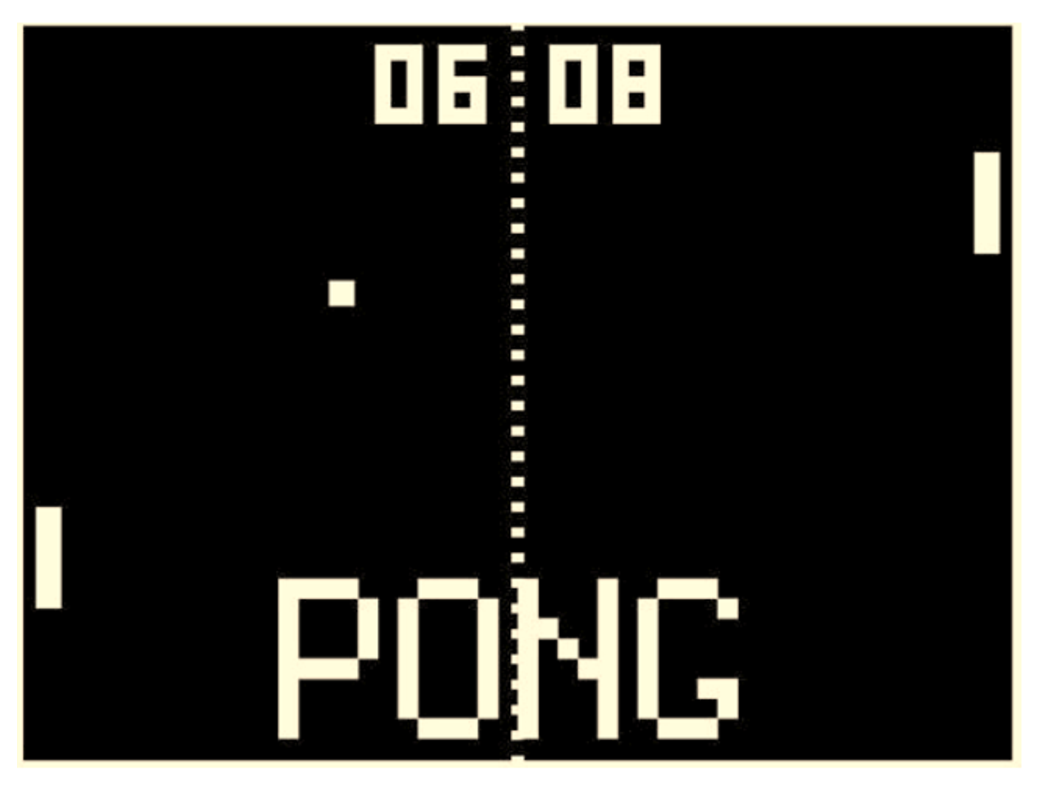
\includegraphics{../Bilder/Bild64-1.eps}}
\end{center}
\begin{scriptsize} Bildquelle: http://www.overclockers.at/games\_forum/euer-erstes-computerspiel\_237146/page\_2 [15.10.2015]. \end{scriptsize}

\begin{center}
	\resizebox{0.5\linewidth}{!}{\newrgbcolor{qqwuqq}{0. 0.39215686274509803 0.}
\psset{xunit=1.0cm,yunit=1.0cm,algebraic=true,dimen=middle,dotstyle=o,dotsize=4pt 0,linewidth=0.8pt,arrowsize=3pt 2,arrowinset=0.25}
\begin{pspicture*}(0.66,5.447272727272732)(8.9,8.537922077922087)
\multips(0,5)(0,1.0){4}{\psline[linestyle=dashed,linecap=1,dash=1.5pt 1.5pt,linewidth=0.4pt,linecolor=lightgray]{c-c}(0.66,0)(8.9,0)}
\multips(0,0)(1.0,0){9}{\psline[linestyle=dashed,linecap=1,dash=1.5pt 1.5pt,linewidth=0.4pt,linecolor=lightgray]{c-c}(0,5.447272727272732)(0,8.537922077922087)}
\psaxes[labelFontSize=\scriptstyle,xAxis=true,yAxis=true,Dx=1.,Dy=1.,ticksize=-2pt 0,subticks=2]{->}(0,0)(0.66,5.447272727272732)(8.9,8.537922077922087)
\psplot[linewidth=0.8pt]{0.66}{8.9}{(--56.-0.*x)/7.}
\psline[linewidth=0.8pt]{->}(5.,8.)(8.,6.)
\psline[linewidth=0.8pt]{->}(2.,6.)(5.,8.)
\pscustom[linewidth=0.8pt,linecolor=qqwuqq,fillcolor=qqwuqq,fillstyle=solid,opacity=0.1]{
\parametricplot{-0.5880026035475675}{0.0}{1.4*cos(t)+5.|1.4*sin(t)+8.}
\lineto(5.,8.)\closepath}
\pscustom[linewidth=0.8pt,linecolor=qqwuqq,fillcolor=qqwuqq,fillstyle=solid,opacity=0.1]{
\parametricplot{3.141592653589793}{3.7295952571373605}{1.4*cos(t)+5.|1.4*sin(t)+8.}
\lineto(5.,8.)\closepath}
\rput[bl](5.8,7.5){\qqwuqq{$\beta$}}
\rput[bl](3.9,7.58){\qqwuqq{$\alpha$}}
\end{pspicture*}}
\end{center}

\subsection{Aufgabenstellung:}
\begin{enumerate}
	\item In einer konkreten Spielsituation hat der Ball beim Aufprall auf den oberen Spielfeldrand einen Geschwindigkeitsvektor von $\vec{v}=\binom{4}{7}$ Pixeln pro Bildaufbau.
	
	\fbox{A} Gib denjenigen Winkel $\alpha$ an, unter dem der Ball auf den Spielfeldrand trifft!
	
	$\alpha$= \rule{5cm}{0.3pt}
	
	Die Komponenten des Geschwindigkeitsvektors sind immer ganzzahlig. Nehmen Sie an, dass die Summe der Beträge der Komponenten nicht größer als 20 sein darf.
	
	Der Ball wird am oberen Spielfeldrand unter dem Winkel $\beta$ reflektiert. Welchen kleinstmöglichen Wert $\beta_\text{min}$ kann unter diesen Voraussetzungen der Winkel $\beta$ annehmen? Gib $\beta_\text{min}$ an!
	
	$\beta_\text{min}$= \rule{5cm}{0.3pt}
	
	\item In einem anderen Spielverlauf befindet sich der Ball im Punkt $(401|301)$ und sein Geschwindigkeitsvektor ist dabei $\vec{v}=\binom{2}{-3}$ Pixel pro Bildaufbau.
	
	Gib an, wie viele \textit{Sekunden} es dauert, bis der Ball am unteren Spielfeldrand reflektiert wird.
	
	Nach dieser Reflexion bewegt sich der Ball entlang einer Geraden bis zum nächsten Auftreffen auf den Schläger oder den Spielfeldrand.
	
 Gib eine Parameterdarstellung dieser Geraden an! 

\item Zwei Kinder, Nicola und Florian, spielen über einen längeren Zeitraum oft gegeneinander \textit{Pong}. Von 45 Spielen gewinnt Nicola 31-mal, Florian gewinnt 14-mal.
 
		Gib auf Basis dieser Information ein symmetrisches $95-\%-$Konfidenzintervall für Nicolas Gewinnwahrscheinlichkeit an!
		
		Erkläre, wieso es nicht sinnvoll ist, ein 100-\%-Konfidenzintervall zu bestimmen!
\end{enumerate}
\antwort{
\begin{enumerate}
	\item \subsection{Lösungserwartung:} 
	
$\tan(\alpha)=\frac{7}{4}=1,74$

$\alpha\approx 60,26^\circ$

Unter diesen Bedingungen lautet der Geschwindigkeitsvektor $\vec{v}= \binom{\pm\,19}{\pm\,1}$ Pixel pro Bildaufbau. Für den Winkel $\beta_\text{min}$ gibt das in jedem Fall:

 $\tan(\beta_\text{min})=\frac{1}{19}$

 $\beta_\text{min}\approx 3,01^\circ$

	\subsection{Lösungsschlüssel:}
	\begin{itemize}
		\item Ein Ausgleichspunkt für die richtige Lösung, wobei die Einheit "`Grad"' nicht angegeben sein muss. Eine korrekte Angabe der Lösung in einer anderen Einheit ist ebenfalls als richtig zu werten. 
		
		Toleranzintervall: $[6011^\circ; 60,3^\circ]$
		\item Ein Punkt für die richtige Lösung, wobei die Einheit "`Grad"' nicht angegeben sein muss. Eine korrekte Angabe der Lösung in einer anderen Einheit ist ebenfalls als richtig zu werten. 
		
		Toleranzintervall: $[3^\circ; 3,02^\circ]$
	\end{itemize}
	
	\item \subsection{Lösungserwartung:}
			
	$301-3n=1 \Rightarrow n=100$
	
	$100\cdot 0,02=2$
	
	Es dauert zwei Sekunden, bis der Ball am unteren Spielfeldrand reflektiert wird.\leer
	
	$g: X=\binom{601}{1}+s\cdot\binom{2}{3}$

	\subsection{Lösungsschlüssel:}
	
\begin{itemize}
	\item Ein Punkt für die richtige Lösung. 
	
	Toleranzintervall: $[2\,\text{s}; 2,02\,\text{s}]$
	\item Ein Punkt für eine korrekte Parameterdarstellung bzw. Gleichung der Geraden. Äquivalente Parameterdarstellungen bzw. Gleichungen sind als richtig zu werten. 
\end{itemize}

\item \subsection{Lösungserwartung:}
			
$n=45, h=\frac{31}{45}$

$\frac{31}{45}\,\pm\,1,96\cdot\sqrt{\frac{\frac{31}{45}\cdot\frac{14}{45}}{45}}\approx 0,689\,\pm\,0,135 \Rightarrow [0,554;0,824]$\leer

Mögliche Erklärungen:

Es ist nicht sinnvoll, ein 100-\%-Konfidenzintervall zu bilden, da die Intervallgrenzen dann 0\,\% bis 100\.\% wären, man hätte also keinen Informationsgewinn. 

 oder:  

 Ein 100-\%-Konfidenzintervall erstreckt sich über den gesamten Definitionsbereich.
	\subsection{Lösungsschlüssel:}
	
\begin{itemize}
	\item Ein Punkt für ein korrektes Intervall. Andere Schreibweisen des Ergebnisses (als Bruch oder in Prozent) sind ebenfalls als richtig zu werten. 
	
	Toleranzintervall für den unteren Wert: $[0,54; 0,56]$ 
	
	Toleranzintervall für den oberen Wert: $[0,81; 0,83]$ 
	
	Die Aufgabe ist auch dann als richtig gelöst zu werten, wenn bei korrektem Ansatz das Ergebnis aufgrund eines Rechenfehlers nicht richtig ist. 
	\item Ein Punkt für eine (sinngemäß) korrekte Erklärung.
\end{itemize}
\end{enumerate}}
		\end{langesbeispiel}